\documentclass[twoside]{book}

% Packages required by doxygen
\usepackage{fixltx2e}
\usepackage{calc}
\usepackage{doxygen}
\usepackage[export]{adjustbox} % also loads graphicx
\usepackage{graphicx}
\usepackage[utf8]{inputenc}
\usepackage{makeidx}
\usepackage{multicol}
\usepackage{multirow}
\PassOptionsToPackage{warn}{textcomp}
\usepackage{textcomp}
\usepackage[nointegrals]{wasysym}
\usepackage[table]{xcolor}

% Font selection
\usepackage[T1]{fontenc}
\usepackage[scaled=.90]{helvet}
\usepackage{courier}
\usepackage{amssymb}
\usepackage{sectsty}
\renewcommand{\familydefault}{\sfdefault}
\allsectionsfont{%
  \fontseries{bc}\selectfont%
  \color{darkgray}%
}
\renewcommand{\DoxyLabelFont}{%
  \fontseries{bc}\selectfont%
  \color{darkgray}%
}
\newcommand{\+}{\discretionary{\mbox{\scriptsize$\hookleftarrow$}}{}{}}

% Page & text layout
\usepackage{geometry}
\geometry{%
  a4paper,%
  top=2.5cm,%
  bottom=2.5cm,%
  left=2.5cm,%
  right=2.5cm%
}
\tolerance=750
\hfuzz=15pt
\hbadness=750
\setlength{\emergencystretch}{15pt}
\setlength{\parindent}{0cm}
\setlength{\parskip}{3ex plus 2ex minus 2ex}
\makeatletter
\renewcommand{\paragraph}{%
  \@startsection{paragraph}{4}{0ex}{-1.0ex}{1.0ex}{%
    \normalfont\normalsize\bfseries\SS@parafont%
  }%
}
\renewcommand{\subparagraph}{%
  \@startsection{subparagraph}{5}{0ex}{-1.0ex}{1.0ex}{%
    \normalfont\normalsize\bfseries\SS@subparafont%
  }%
}
\makeatother

% Headers & footers
\usepackage{fancyhdr}
\pagestyle{fancyplain}
\fancyhead[LE]{\fancyplain{}{\bfseries\thepage}}
\fancyhead[CE]{\fancyplain{}{}}
\fancyhead[RE]{\fancyplain{}{\bfseries\leftmark}}
\fancyhead[LO]{\fancyplain{}{\bfseries\rightmark}}
\fancyhead[CO]{\fancyplain{}{}}
\fancyhead[RO]{\fancyplain{}{\bfseries\thepage}}
\fancyfoot[LE]{\fancyplain{}{}}
\fancyfoot[CE]{\fancyplain{}{}}
\fancyfoot[RE]{\fancyplain{}{\bfseries\scriptsize Generated by Doxygen }}
\fancyfoot[LO]{\fancyplain{}{\bfseries\scriptsize Generated by Doxygen }}
\fancyfoot[CO]{\fancyplain{}{}}
\fancyfoot[RO]{\fancyplain{}{}}
\renewcommand{\footrulewidth}{0.4pt}
\renewcommand{\chaptermark}[1]{%
  \markboth{#1}{}%
}
\renewcommand{\sectionmark}[1]{%
  \markright{\thesection\ #1}%
}

% Indices & bibliography
\usepackage{natbib}
\usepackage[titles]{tocloft}
\setcounter{tocdepth}{3}
\setcounter{secnumdepth}{5}
\makeindex

% Hyperlinks (required, but should be loaded last)
\usepackage{ifpdf}
\ifpdf
  \usepackage[pdftex,pagebackref=true]{hyperref}
\else
  \usepackage[ps2pdf,pagebackref=true]{hyperref}
\fi
\hypersetup{%
  colorlinks=true,%
  linkcolor=blue,%
  citecolor=blue,%
  unicode%
}

% Custom commands
\newcommand{\clearemptydoublepage}{%
  \newpage{\pagestyle{empty}\cleardoublepage}%
}

\usepackage{caption}
\captionsetup{labelsep=space,justification=centering,font={bf},singlelinecheck=off,skip=4pt,position=top}

%===== C O N T E N T S =====

\begin{document}

% Titlepage & ToC
\hypersetup{pageanchor=false,
             bookmarksnumbered=true,
             pdfencoding=unicode
            }
\pagenumbering{alph}
\begin{titlepage}
\vspace*{7cm}
\begin{center}%
{\Large Structure Factor, R\+DF Analysis }\\
\vspace*{1cm}
{\large Generated by Doxygen 1.8.14}\\
\end{center}
\end{titlepage}
\clearemptydoublepage
\pagenumbering{roman}
\tableofcontents
\clearemptydoublepage
\pagenumbering{arabic}
\hypersetup{pageanchor=true}

%--- Begin generated contents ---
\chapter{structure\+Factor}
\label{md_README}
\Hypertarget{md_README}
Post-\/processing code for R\+DF, in-\/plane R\+DF, structure factor

This C++ program reads in lammps trajectory files or X\+YZ files to calculate R\+DF, in-\/plane R\+DF and the structure factor.

\section*{Compilation}

To generate the executable {\itshape runme} use\+:


\begin{DoxyCode}{0}
\DoxyCodeLine{make }
\end{DoxyCode}


An executable {\itshape runme} will be formed in the base directory.

\section*{Running}


\begin{DoxyCode}{0}
\DoxyCodeLine{./runme}
\end{DoxyCode}


\section*{Details}


\begin{DoxyItemize}
\item For example, if you want to find the in-\/plane R\+DF in the XY plane, you should use the \mbox{\hyperlink{classRdf2D}{Rdf2D}} class. The equation used for 2D-\/\+R\+DF for the $n^{th}$ layer is\+: \[ g^n(r) = \frac{1}{(\rho^n)^2 A \delta z} \Sigma_{i \neq j} \delta(r - r_{ij}) \left[ \Theta\left( \frac{\delta z}{2}-|z_i-z^2| \right) \times \Theta\left( \frac{\delta z}{2}-|z_j-z^n| \right) \right] \] For detailed instructions, see the \mbox{\hyperlink{classRdf2D}{Rdf2D}} class documentation 
\end{DoxyItemize}
\chapter{Hierarchical Index}
\section{Class Hierarchy}
This inheritance list is sorted roughly, but not completely, alphabetically\+:\begin{DoxyCompactList}
\item \contentsline{section}{C\+Molecular\+System}{\pageref{classCMolecularSystem}}{}
\item \contentsline{section}{C\+Molecule}{\pageref{classCMolecule}}{}
\item \contentsline{section}{C\+Output}{\pageref{classCOutput}}{}
\begin{DoxyCompactList}
\item \contentsline{section}{Rdf3D}{\pageref{classRdf3D}}{}
\end{DoxyCompactList}
\item \contentsline{section}{C\+Parameter}{\pageref{classCParameter}}{}
\item \contentsline{section}{Exception\+Bad\+Line\+In\+Parameter\+File}{\pageref{classExceptionBadLineInParameterFile}}{}
\item \contentsline{section}{Number\+Of\+Particles\+Not\+Defined\+Exception}{\pageref{classNumberOfParticlesNotDefinedException}}{}
\item \contentsline{section}{s\+\_\+raw\+Parameter}{\pageref{structs__rawParameter}}{}
\end{DoxyCompactList}

\chapter{Class Index}
\section{Class List}
Here are the classes, structs, unions and interfaces with brief descriptions\+:\begin{DoxyCompactList}
\item\contentsline{section}{\mbox{\hyperlink{classCAnalysis}{C\+Analysis}} }{\pageref{classCAnalysis}}{}
\item\contentsline{section}{\mbox{\hyperlink{classCMolecularSystem}{C\+Molecular\+System}} }{\pageref{classCMolecularSystem}}{}
\item\contentsline{section}{\mbox{\hyperlink{classCMolecule}{C\+Molecule}} }{\pageref{classCMolecule}}{}
\item\contentsline{section}{\mbox{\hyperlink{classCOutput}{C\+Output}} }{\pageref{classCOutput}}{}
\item\contentsline{section}{\mbox{\hyperlink{classCParameter}{C\+Parameter}} }{\pageref{classCParameter}}{}
\item\contentsline{section}{\mbox{\hyperlink{classExceptionBadLineInParameterFile}{Exception\+Bad\+Line\+In\+Parameter\+File}} }{\pageref{classExceptionBadLineInParameterFile}}{}
\item\contentsline{section}{\mbox{\hyperlink{classNumberOfParticlesNotDefinedException}{Number\+Of\+Particles\+Not\+Defined\+Exception}} }{\pageref{classNumberOfParticlesNotDefinedException}}{}
\item\contentsline{section}{\mbox{\hyperlink{structs__rawParameter}{s\+\_\+raw\+Parameter}} }{\pageref{structs__rawParameter}}{}
\end{DoxyCompactList}

\chapter{Class Documentation}
\hypertarget{classCMolecularSystem}{}\section{C\+Molecular\+System Class Reference}
\label{classCMolecularSystem}\index{C\+Molecular\+System@{C\+Molecular\+System}}
\subsection*{Public Member Functions}
\begin{DoxyCompactItemize}
\item 
\mbox{\Hypertarget{classCMolecularSystem_afcebd0d1032cbe262c82825ceb78b4a5}\label{classCMolecularSystem_afcebd0d1032cbe262c82825ceb78b4a5}} 
void {\bfseries initialize\+Molecules} (int)
\item 
\mbox{\Hypertarget{classCMolecularSystem_a3635729781d41229ce16fabea4ce9b6f}\label{classCMolecularSystem_a3635729781d41229ce16fabea4ce9b6f}} 
void {\bfseries initialize\+Molecules} ()
\item 
\mbox{\Hypertarget{classCMolecularSystem_a5a31541d610fe40d42a31283eb9a8845}\label{classCMolecularSystem_a5a31541d610fe40d42a31283eb9a8845}} 
void {\bfseries delete\+Molecules} ()
\item 
\mbox{\Hypertarget{classCMolecularSystem_a9084e19d4554f70ae7e603c7cab3a2ae}\label{classCMolecularSystem_a9084e19d4554f70ae7e603c7cab3a2ae}} 
void {\bfseries Initialize\+System} ()
\item 
\mbox{\Hypertarget{classCMolecularSystem_a019709e83f903659bdb82c226da4189a}\label{classCMolecularSystem_a019709e83f903659bdb82c226da4189a}} 
void {\bfseries read\+Particle\+File} ()
\item 
\mbox{\Hypertarget{classCMolecularSystem_a68c2be35fb9f9dbd1915ddf1c845eb15}\label{classCMolecularSystem_a68c2be35fb9f9dbd1915ddf1c845eb15}} 
void {\bfseries read\+Whole\+Trj} ()
\item 
\mbox{\Hypertarget{classCMolecularSystem_a7ccd08c6a0182faf0316d9f1f8ec1651}\label{classCMolecularSystem_a7ccd08c6a0182faf0316d9f1f8ec1651}} 
void {\bfseries read\+Particle\+File} (int)
\end{DoxyCompactItemize}
\subsection*{Public Attributes}
\begin{DoxyCompactItemize}
\item 
\mbox{\Hypertarget{classCMolecularSystem_a1431a8bd6aa95b62a025afdca53d9e1c}\label{classCMolecularSystem_a1431a8bd6aa95b62a025afdca53d9e1c}} 
\mbox{\hyperlink{classCMolecule}{C\+Molecule}} $\ast$ {\bfseries molecules}
\item 
\mbox{\Hypertarget{classCMolecularSystem_a4139e417a2b508576800fc44ce691db2}\label{classCMolecularSystem_a4139e417a2b508576800fc44ce691db2}} 
\mbox{\hyperlink{classCParameter}{C\+Parameter}} $\ast$ {\bfseries parameter}
\end{DoxyCompactItemize}


The documentation for this class was generated from the following files\+:\begin{DoxyCompactItemize}
\item 
molecular\+\_\+system.\+h\item 
molecular\+\_\+system.\+cpp\end{DoxyCompactItemize}

\hypertarget{classCMolecule}{}\section{C\+Molecule Class Reference}
\label{classCMolecule}\index{C\+Molecule@{C\+Molecule}}
\subsection*{Public Member Functions}
\begin{DoxyCompactItemize}
\item 
\mbox{\hyperlink{classCMolecule_a6e4328f4451a293bb1405bbde90a4ced}{C\+Molecule}} ()
\item 
virtual \mbox{\hyperlink{classCMolecule_a8e59e7e7ff05b619a9e201c3263921c5}{$\sim$\+C\+Molecule}} ()
\item 
void \mbox{\hyperlink{classCMolecule_ad9a66ae676bd9ed1012f0c6e952369e0}{set\+\_\+position}} (double, double, double)
\item 
double \mbox{\hyperlink{classCMolecule_ac76dbb1e5abbc9fbadcd568d0f2e7d16}{get\+\_\+posx}} ()
\item 
double \mbox{\hyperlink{classCMolecule_a8cf1a6b995c8cbf4f1881f6f38ebca02}{get\+\_\+posy}} ()
\item 
double \mbox{\hyperlink{classCMolecule_a69483e3d6820a96f004ba6c78f8d166e}{get\+\_\+posz}} ()
\end{DoxyCompactItemize}
\subsection*{Public Attributes}
\begin{DoxyCompactItemize}
\item 
\mbox{\Hypertarget{classCMolecule_adfbd57e11262264d1085003ce6980e0e}\label{classCMolecule_adfbd57e11262264d1085003ce6980e0e}} 
double {\bfseries vx}
\item 
\mbox{\Hypertarget{classCMolecule_a940450fd2115a50185bc25d62d222bfa}\label{classCMolecule_a940450fd2115a50185bc25d62d222bfa}} 
double {\bfseries vy}
\item 
\mbox{\Hypertarget{classCMolecule_a6958f8a29883dcb7c9b95b6d4b672a04}\label{classCMolecule_a6958f8a29883dcb7c9b95b6d4b672a04}} 
double {\bfseries vz}
\item 
\mbox{\Hypertarget{classCMolecule_afdf067ddb470fd2abd5bfd51b725421c}\label{classCMolecule_afdf067ddb470fd2abd5bfd51b725421c}} 
double {\bfseries fx}
\item 
\mbox{\Hypertarget{classCMolecule_ac193b9e1e9a9bba2ac8ec5a92509dc75}\label{classCMolecule_ac193b9e1e9a9bba2ac8ec5a92509dc75}} 
double {\bfseries fy}
\item 
\mbox{\Hypertarget{classCMolecule_a98856c34c33ffbb79dd672f68df7495f}\label{classCMolecule_a98856c34c33ffbb79dd672f68df7495f}} 
double {\bfseries fz}
\item 
\mbox{\Hypertarget{classCMolecule_a8b406afe8e1b88c5ad285fbcab5cf4d0}\label{classCMolecule_a8b406afe8e1b88c5ad285fbcab5cf4d0}} 
double {\bfseries rfx}
\item 
\mbox{\Hypertarget{classCMolecule_a3397d14c0de2638847411f990159f817}\label{classCMolecule_a3397d14c0de2638847411f990159f817}} 
double {\bfseries rfy}
\item 
\mbox{\Hypertarget{classCMolecule_a662bb860661423a13952f53bf347ee0a}\label{classCMolecule_a662bb860661423a13952f53bf347ee0a}} 
double {\bfseries rfz}
\item 
\mbox{\Hypertarget{classCMolecule_ae38677450bdb6d4dacfa739381e30e64}\label{classCMolecule_ae38677450bdb6d4dacfa739381e30e64}} 
double {\bfseries potential}
\item 
\mbox{\Hypertarget{classCMolecule_a5e11f667a1757d5eac1e14090acbbe94}\label{classCMolecule_a5e11f667a1757d5eac1e14090acbbe94}} 
int {\bfseries type}
\end{DoxyCompactItemize}


\subsection{Constructor \& Destructor Documentation}
\mbox{\Hypertarget{classCMolecule_a6e4328f4451a293bb1405bbde90a4ced}\label{classCMolecule_a6e4328f4451a293bb1405bbde90a4ced}} 
\index{C\+Molecule@{C\+Molecule}!C\+Molecule@{C\+Molecule}}
\index{C\+Molecule@{C\+Molecule}!C\+Molecule@{C\+Molecule}}
\subsubsection{\texorpdfstring{C\+Molecule()}{CMolecule()}}
{\footnotesize\ttfamily C\+Molecule\+::\+C\+Molecule (\begin{DoxyParamCaption}{ }\end{DoxyParamCaption})}

Constructor \mbox{\Hypertarget{classCMolecule_a8e59e7e7ff05b619a9e201c3263921c5}\label{classCMolecule_a8e59e7e7ff05b619a9e201c3263921c5}} 
\index{C\+Molecule@{C\+Molecule}!````~C\+Molecule@{$\sim$\+C\+Molecule}}
\index{````~C\+Molecule@{$\sim$\+C\+Molecule}!C\+Molecule@{C\+Molecule}}
\subsubsection{\texorpdfstring{$\sim$\+C\+Molecule()}{~CMolecule()}}
{\footnotesize\ttfamily C\+Molecule\+::$\sim$\+C\+Molecule (\begin{DoxyParamCaption}{ }\end{DoxyParamCaption})\hspace{0.3cm}{\ttfamily [virtual]}}

Destructor 

\subsection{Member Function Documentation}
\mbox{\Hypertarget{classCMolecule_ac76dbb1e5abbc9fbadcd568d0f2e7d16}\label{classCMolecule_ac76dbb1e5abbc9fbadcd568d0f2e7d16}} 
\index{C\+Molecule@{C\+Molecule}!get\+\_\+posx@{get\+\_\+posx}}
\index{get\+\_\+posx@{get\+\_\+posx}!C\+Molecule@{C\+Molecule}}
\subsubsection{\texorpdfstring{get\+\_\+posx()}{get\_posx()}}
{\footnotesize\ttfamily double C\+Molecule\+::get\+\_\+posx (\begin{DoxyParamCaption}{ }\end{DoxyParamCaption})}

Get the x-\/\+Component of the position \mbox{\Hypertarget{classCMolecule_a8cf1a6b995c8cbf4f1881f6f38ebca02}\label{classCMolecule_a8cf1a6b995c8cbf4f1881f6f38ebca02}} 
\index{C\+Molecule@{C\+Molecule}!get\+\_\+posy@{get\+\_\+posy}}
\index{get\+\_\+posy@{get\+\_\+posy}!C\+Molecule@{C\+Molecule}}
\subsubsection{\texorpdfstring{get\+\_\+posy()}{get\_posy()}}
{\footnotesize\ttfamily double C\+Molecule\+::get\+\_\+posy (\begin{DoxyParamCaption}{ }\end{DoxyParamCaption})}

Get the y-\/\+Component of the position \mbox{\Hypertarget{classCMolecule_a69483e3d6820a96f004ba6c78f8d166e}\label{classCMolecule_a69483e3d6820a96f004ba6c78f8d166e}} 
\index{C\+Molecule@{C\+Molecule}!get\+\_\+posz@{get\+\_\+posz}}
\index{get\+\_\+posz@{get\+\_\+posz}!C\+Molecule@{C\+Molecule}}
\subsubsection{\texorpdfstring{get\+\_\+posz()}{get\_posz()}}
{\footnotesize\ttfamily double C\+Molecule\+::get\+\_\+posz (\begin{DoxyParamCaption}{ }\end{DoxyParamCaption})}

Get the z-\/\+Component of the position \mbox{\Hypertarget{classCMolecule_ad9a66ae676bd9ed1012f0c6e952369e0}\label{classCMolecule_ad9a66ae676bd9ed1012f0c6e952369e0}} 
\index{C\+Molecule@{C\+Molecule}!set\+\_\+position@{set\+\_\+position}}
\index{set\+\_\+position@{set\+\_\+position}!C\+Molecule@{C\+Molecule}}
\subsubsection{\texorpdfstring{set\+\_\+position()}{set\_position()}}
{\footnotesize\ttfamily void C\+Molecule\+::set\+\_\+position (\begin{DoxyParamCaption}\item[{double}]{x,  }\item[{double}]{y,  }\item[{double}]{z }\end{DoxyParamCaption})}

Sets the position of the molecule 

The documentation for this class was generated from the following files\+:\begin{DoxyCompactItemize}
\item 
molecule.\+h\item 
molecule.\+cpp\end{DoxyCompactItemize}

\hypertarget{classCOutput}{}\section{C\+Output Class Reference}
\label{classCOutput}\index{C\+Output@{C\+Output}}
Inheritance diagram for C\+Output\+:\begin{figure}[H]
\begin{center}
\leavevmode
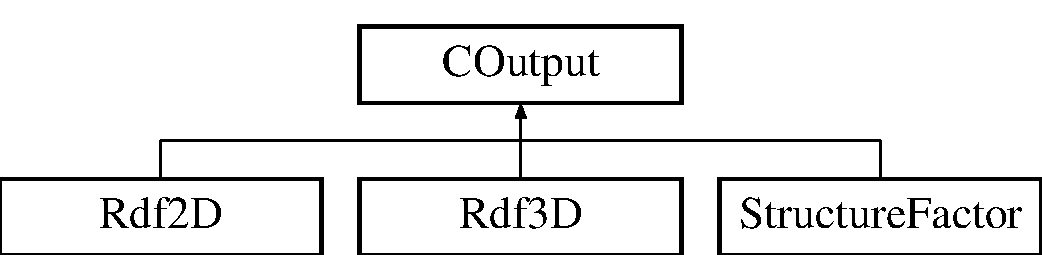
\includegraphics[height=2.000000cm]{classCOutput}
\end{center}
\end{figure}
\subsection*{Public Member Functions}
\begin{DoxyCompactItemize}
\item 
\mbox{\Hypertarget{classCOutput_a01760ac1e3f30b98ebfd768e3e100e87}\label{classCOutput_a01760ac1e3f30b98ebfd768e3e100e87}} 
void {\bfseries print\+To\+File} (int, double $\ast$x, double $\ast$y, const std\+::string \&filename=\char`\"{}output\char`\"{}, const std\+::string \&x\+Name=\char`\"{}Abscissa\char`\"{}, const std\+::string \&y\+Name=\char`\"{}Ordinate\char`\"{})
\item 
\mbox{\Hypertarget{classCOutput_a166f58fa47dc422665a223974e707241}\label{classCOutput_a166f58fa47dc422665a223974e707241}} 
void {\bfseries create\+Output\+Dir} (const char $\ast$path)
\end{DoxyCompactItemize}


The documentation for this class was generated from the following files\+:\begin{DoxyCompactItemize}
\item 
output.\+h\item 
output.\+cpp\end{DoxyCompactItemize}

\hypertarget{classCParameter}{}\section{C\+Parameter Class Reference}
\label{classCParameter}\index{C\+Parameter@{C\+Parameter}}
\subsection*{Public Member Functions}
\begin{DoxyCompactItemize}
\item 
\mbox{\Hypertarget{classCParameter_a026d8da357935e384b478913e036f3bc}\label{classCParameter_a026d8da357935e384b478913e036f3bc}} 
void {\bfseries read\+Parameter} ()
\end{DoxyCompactItemize}
\subsection*{Public Attributes}
\begin{DoxyCompactItemize}
\item 
\mbox{\Hypertarget{classCParameter_a8c3dd5e12ba81bf46bce96e7172f08d6}\label{classCParameter_a8c3dd5e12ba81bf46bce96e7172f08d6}} 
\mbox{\hyperlink{structs__rawParameter}{s\+\_\+raw\+Parameter}} {\bfseries raw\+Parameter} \mbox{[}N\+U\+M\+B\+E\+R\+\_\+\+O\+F\+\_\+\+P\+A\+R\+A\+M\+E\+T\+E\+RS\mbox{]}
\item 
\mbox{\Hypertarget{classCParameter_adce9321ac8e877aff4d4c9fc03f74465}\label{classCParameter_adce9321ac8e877aff4d4c9fc03f74465}} 
int {\bfseries nop}
\item 
\mbox{\Hypertarget{classCParameter_ab0abbb096d718eb1deac73e1c47ae324}\label{classCParameter_ab0abbb096d718eb1deac73e1c47ae324}} 
double {\bfseries boxx}
\item 
\mbox{\Hypertarget{classCParameter_af770455c1829b9e2ab5cd27b7ea626be}\label{classCParameter_af770455c1829b9e2ab5cd27b7ea626be}} 
double {\bfseries boxy}
\item 
\mbox{\Hypertarget{classCParameter_a87d3e3cd240bb45c5d9dcbd6c3cc3bf0}\label{classCParameter_a87d3e3cd240bb45c5d9dcbd6c3cc3bf0}} 
double {\bfseries boxz}
\item 
\mbox{\Hypertarget{classCParameter_ace7b05009f3403d4abea8a1bea18ded8}\label{classCParameter_ace7b05009f3403d4abea8a1bea18ded8}} 
std\+::string {\bfseries xyz\+File}
\item 
\mbox{\Hypertarget{classCParameter_a0b417a4a872ded310baf1c310f55c284}\label{classCParameter_a0b417a4a872ded310baf1c310f55c284}} 
std\+::string {\bfseries traj\+File}
\item 
\mbox{\Hypertarget{classCParameter_a0d4870d1e8738b7d921e35fa4068b060}\label{classCParameter_a0d4870d1e8738b7d921e35fa4068b060}} 
int {\bfseries nsteps}
\end{DoxyCompactItemize}


The documentation for this class was generated from the following files\+:\begin{DoxyCompactItemize}
\item 
parameter.\+h\item 
parameter.\+cpp\end{DoxyCompactItemize}

\hypertarget{classExceptionBadLineInParameterFile}{}\section{Exception\+Bad\+Line\+In\+Parameter\+File Class Reference}
\label{classExceptionBadLineInParameterFile}\index{Exception\+Bad\+Line\+In\+Parameter\+File@{Exception\+Bad\+Line\+In\+Parameter\+File}}


The documentation for this class was generated from the following file\+:\begin{DoxyCompactItemize}
\item 
parameter.\+h\end{DoxyCompactItemize}

\hypertarget{classNumberOfParticlesNotDefinedException}{}\section{Number\+Of\+Particles\+Not\+Defined\+Exception Class Reference}
\label{classNumberOfParticlesNotDefinedException}\index{Number\+Of\+Particles\+Not\+Defined\+Exception@{Number\+Of\+Particles\+Not\+Defined\+Exception}}


The documentation for this class was generated from the following file\+:\begin{DoxyCompactItemize}
\item 
molecular\+\_\+system.\+h\end{DoxyCompactItemize}

\hypertarget{classRdf2D}{}\section{Rdf2D Class Reference}
\label{classRdf2D}\index{Rdf2D@{Rdf2D}}


Class for 2D R\+DF. This class creates an object for the 2D-\/\+R\+DF, and the output of the R\+DF can be printed to a file.  




{\ttfamily \#include $<$rdf2\+D.\+h$>$}

Inheritance diagram for Rdf2D\+:\begin{figure}[H]
\begin{center}
\leavevmode
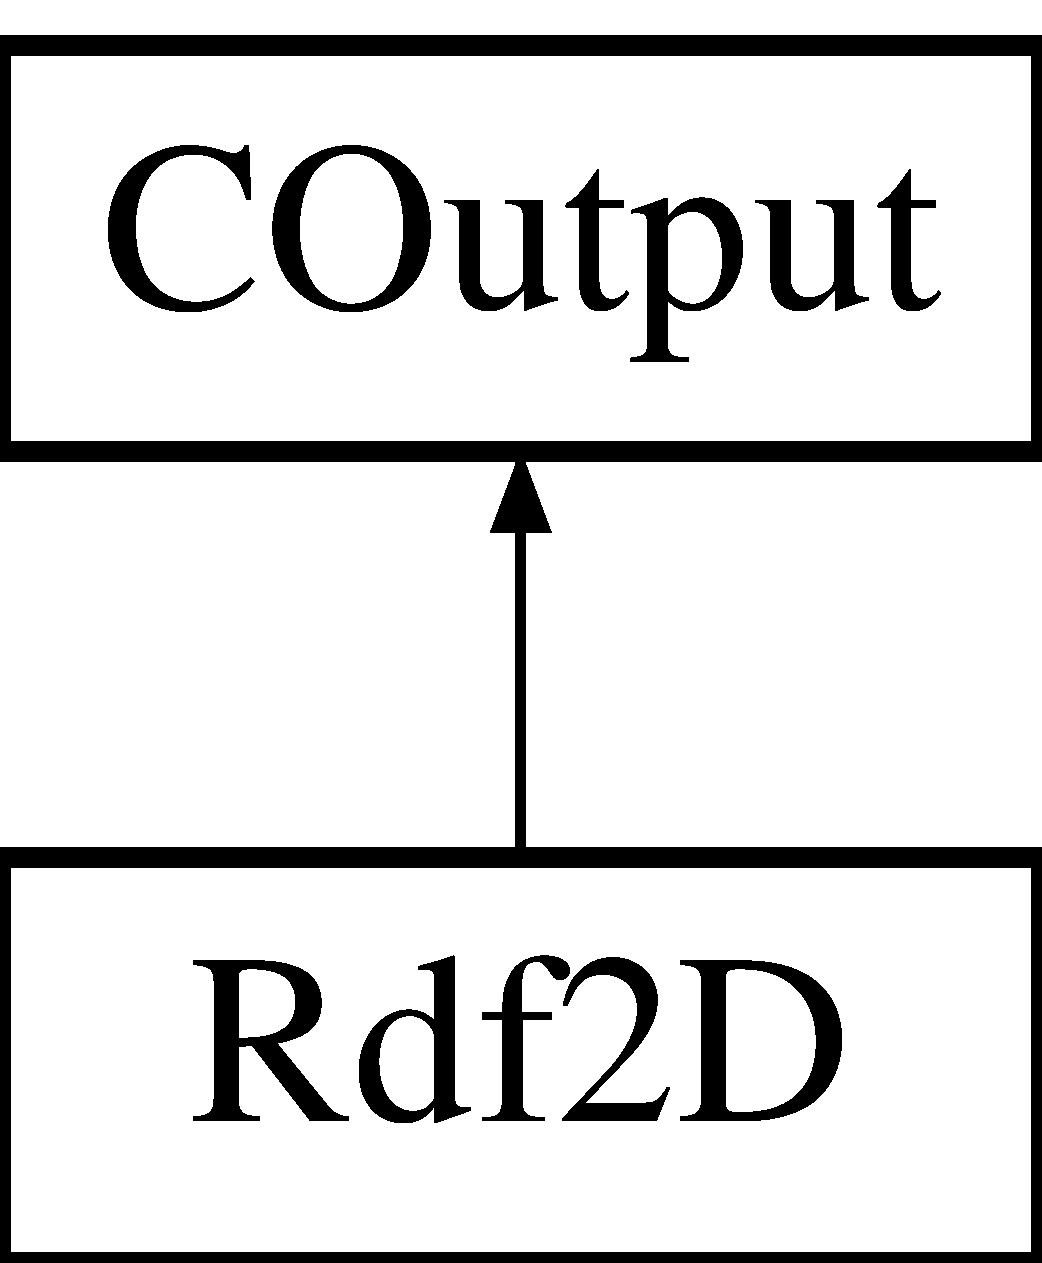
\includegraphics[height=2.000000cm]{classRdf2D}
\end{center}
\end{figure}
\subsection*{Public Member Functions}
\begin{DoxyCompactItemize}
\item 
void \mbox{\hyperlink{classRdf2D_a767f006de6412394a59f1cae5f7f6b35}{init\+R\+D\+Fxy}} (class \mbox{\hyperlink{classCMolecularSystem}{C\+Molecular\+System}} \&mol\+Sys, double binwidth, double volume=-\/1.\+0, double max\+\_\+radius=-\/1.\+0)
\item 
void \mbox{\hyperlink{classRdf2D_afc5ff73aa9c126184e94ee3abfc14ff4}{single\+R\+D\+Fxy}} (class \mbox{\hyperlink{classCMolecularSystem}{C\+Molecular\+System}} \&mol\+Sys, double z\+\_\+layer, double dz, int typeA=-\/1, int typeB=-\/1)
\item 
void \mbox{\hyperlink{classRdf2D_a6c716851d80fd2a7dcfefd219892d87b}{accumulate\+R\+D\+Fxy}} (class \mbox{\hyperlink{classCMolecularSystem}{C\+Molecular\+System}} \&mol\+Sys, double z\+\_\+layer, double dz, int typeA=-\/1, int typeB=-\/1)
\item 
void \mbox{\hyperlink{classRdf2D_acf73dc86f20e82799157ff53994a2754}{normalize\+R\+D\+F2D}} (double)
\item 
void \mbox{\hyperlink{classRdf2D_a3c8153b303733b7e5d320f9b20f37b32}{getR}} ()
\item 
void \mbox{\hyperlink{classRdf2D_a9658a9bb2229afda0d743bdc05a27411}{clear\+R\+D\+F2D}} ()
\item 
void \mbox{\hyperlink{classRdf2D_aae00c1526117f6ac63d2c13354b6c404}{print\+R\+D\+F2D}} ()
\item 
void \mbox{\hyperlink{classRdf2D_a8008421c8aedff5887160b455879d36b}{delete\+R\+D\+F2D}} ()
\end{DoxyCompactItemize}
\subsection*{Public Attributes}
\begin{DoxyCompactItemize}
\item 
\mbox{\Hypertarget{classRdf2D_ad756caf75c389a69754105c70fb5db60}\label{classRdf2D_ad756caf75c389a69754105c70fb5db60}} 
double $\ast$ {\bfseries rdf2D}
\item 
\mbox{\Hypertarget{classRdf2D_a3f7fdb2bb7ba36ff77f721c4abc8120a}\label{classRdf2D_a3f7fdb2bb7ba36ff77f721c4abc8120a}} 
double $\ast$ {\bfseries r\+Val}
\item 
\mbox{\Hypertarget{classRdf2D_a5720844aa069901d9e3b91a943af4ed8}\label{classRdf2D_a5720844aa069901d9e3b91a943af4ed8}} 
int {\bfseries typeA}
\item 
\mbox{\Hypertarget{classRdf2D_ac4301eef0e368e8b67b6d03a152e0e8b}\label{classRdf2D_ac4301eef0e368e8b67b6d03a152e0e8b}} 
int {\bfseries typeB}
\end{DoxyCompactItemize}


\subsection{Detailed Description}
Class for 2D R\+DF. This class creates an object for the 2D-\/\+R\+DF, and the output of the R\+DF can be printed to a file. 

Use 

\subsection{Member Function Documentation}
\mbox{\Hypertarget{classRdf2D_a6c716851d80fd2a7dcfefd219892d87b}\label{classRdf2D_a6c716851d80fd2a7dcfefd219892d87b}} 
\index{Rdf2D@{Rdf2D}!accumulate\+R\+D\+Fxy@{accumulate\+R\+D\+Fxy}}
\index{accumulate\+R\+D\+Fxy@{accumulate\+R\+D\+Fxy}!Rdf2D@{Rdf2D}}
\subsubsection{\texorpdfstring{accumulate\+R\+D\+Fxy()}{accumulateRDFxy()}}
{\footnotesize\ttfamily void Rdf2\+D\+::accumulate\+R\+D\+Fxy (\begin{DoxyParamCaption}\item[{class \mbox{\hyperlink{classCMolecularSystem}{C\+Molecular\+System}} \&}]{mol\+Sys,  }\item[{double}]{z\+\_\+layer,  }\item[{double}]{dz,  }\item[{int}]{typeA = {\ttfamily -\/1},  }\item[{int}]{typeB = {\ttfamily -\/1} }\end{DoxyParamCaption})}

Calculates the 2D radial distribution function for a number of snapshots for a particular XY plane, specified by a range of z values

It accepts the \mbox{\hyperlink{classCMolecularSystem}{C\+Molecular\+System}} object reference and a pair of int type numbers corresponding to lammps type I\+Ds in the trajectory file, and z\+\_\+min and z\+\_\+max as arguments. If the integer type I\+Ds are not set, then the R\+DF is calculated for all the atoms in the frame, assuming they are all of the same type.

There is no need to use \mbox{\hyperlink{classRdf2D_afc5ff73aa9c126184e94ee3abfc14ff4}{single\+R\+D\+Fxy()}} if the R\+DF is to be calculated over a number of frames. You will have to call the normalize function normalize\+R\+D\+Fxy() separately after accumulating to get the R\+DF \mbox{\Hypertarget{classRdf2D_a9658a9bb2229afda0d743bdc05a27411}\label{classRdf2D_a9658a9bb2229afda0d743bdc05a27411}} 
\index{Rdf2D@{Rdf2D}!clear\+R\+D\+F2D@{clear\+R\+D\+F2D}}
\index{clear\+R\+D\+F2D@{clear\+R\+D\+F2D}!Rdf2D@{Rdf2D}}
\subsubsection{\texorpdfstring{clear\+R\+D\+F2\+D()}{clearRDF2D()}}
{\footnotesize\ttfamily void Rdf2\+D\+::clear\+R\+D\+F2D (\begin{DoxyParamCaption}{ }\end{DoxyParamCaption})}

Sets all the histogram values to zero and sets the number of frames to zero so that the object can be re-\/used. However, the binwidth and maximum radius remain the same. This can be used to re-\/use the object for a different frame etc. Use single\+R\+D\+F3\+D() or accumulate\+R\+D\+F3\+D() after this function \mbox{\Hypertarget{classRdf2D_a8008421c8aedff5887160b455879d36b}\label{classRdf2D_a8008421c8aedff5887160b455879d36b}} 
\index{Rdf2D@{Rdf2D}!delete\+R\+D\+F2D@{delete\+R\+D\+F2D}}
\index{delete\+R\+D\+F2D@{delete\+R\+D\+F2D}!Rdf2D@{Rdf2D}}
\subsubsection{\texorpdfstring{delete\+R\+D\+F2\+D()}{deleteRDF2D()}}
{\footnotesize\ttfamily void Rdf2\+D\+::delete\+R\+D\+F2D (\begin{DoxyParamCaption}{ }\end{DoxyParamCaption})}

Frees the memory \mbox{\Hypertarget{classRdf2D_a3c8153b303733b7e5d320f9b20f37b32}\label{classRdf2D_a3c8153b303733b7e5d320f9b20f37b32}} 
\index{Rdf2D@{Rdf2D}!getR@{getR}}
\index{getR@{getR}!Rdf2D@{Rdf2D}}
\subsubsection{\texorpdfstring{get\+R()}{getR()}}
{\footnotesize\ttfamily void Rdf2\+D\+::getR (\begin{DoxyParamCaption}{ }\end{DoxyParamCaption})}

Get the radial R values corresponding to each R\+DF value This will remain the same over all frames \mbox{\Hypertarget{classRdf2D_a767f006de6412394a59f1cae5f7f6b35}\label{classRdf2D_a767f006de6412394a59f1cae5f7f6b35}} 
\index{Rdf2D@{Rdf2D}!init\+R\+D\+Fxy@{init\+R\+D\+Fxy}}
\index{init\+R\+D\+Fxy@{init\+R\+D\+Fxy}!Rdf2D@{Rdf2D}}
\subsubsection{\texorpdfstring{init\+R\+D\+Fxy()}{initRDFxy()}}
{\footnotesize\ttfamily void Rdf2\+D\+::init\+R\+D\+Fxy (\begin{DoxyParamCaption}\item[{class \mbox{\hyperlink{classCMolecularSystem}{C\+Molecular\+System}} \&}]{mol\+Sys,  }\item[{double}]{binwidth,  }\item[{double}]{volume = {\ttfamily -\/1.0},  }\item[{double}]{max\+\_\+radius = {\ttfamily -\/1.0} }\end{DoxyParamCaption})}

Initializes the histogram array for 2-\/D R\+DF

It takes the \mbox{\hyperlink{classCMolecularSystem}{C\+Molecular\+System}} object reference and binwidth as arguments. Optional arguments include the maximum radius upto which the 3-\/D R\+DF will be calculated and the desired volume. If not set, the default values are half the simulation box and the volume of the simulation box respectively \mbox{\Hypertarget{classRdf2D_acf73dc86f20e82799157ff53994a2754}\label{classRdf2D_acf73dc86f20e82799157ff53994a2754}} 
\index{Rdf2D@{Rdf2D}!normalize\+R\+D\+F2D@{normalize\+R\+D\+F2D}}
\index{normalize\+R\+D\+F2D@{normalize\+R\+D\+F2D}!Rdf2D@{Rdf2D}}
\subsubsection{\texorpdfstring{normalize\+R\+D\+F2\+D()}{normalizeRDF2D()}}
{\footnotesize\ttfamily void Rdf2\+D\+::normalize\+R\+D\+F2D (\begin{DoxyParamCaption}\item[{double}]{dz }\end{DoxyParamCaption})}

Normalizes the R\+DF for the 2D R\+DF

You will have to call this after \mbox{\hyperlink{classRdf2D_a6c716851d80fd2a7dcfefd219892d87b}{accumulate\+R\+D\+Fxy()}} if you are averaging over several snapshots. This is automatically called inside \mbox{\hyperlink{classRdf2D_afc5ff73aa9c126184e94ee3abfc14ff4}{single\+R\+D\+Fxy()}} and other single frame R\+DF functions. This method also accepts the width of the layer as the argument The accuracy of the R\+DF calculation is sensitive to the layer width entered \mbox{\Hypertarget{classRdf2D_aae00c1526117f6ac63d2c13354b6c404}\label{classRdf2D_aae00c1526117f6ac63d2c13354b6c404}} 
\index{Rdf2D@{Rdf2D}!print\+R\+D\+F2D@{print\+R\+D\+F2D}}
\index{print\+R\+D\+F2D@{print\+R\+D\+F2D}!Rdf2D@{Rdf2D}}
\subsubsection{\texorpdfstring{print\+R\+D\+F2\+D()}{printRDF2D()}}
{\footnotesize\ttfamily void Rdf2\+D\+::print\+R\+D\+F2D (\begin{DoxyParamCaption}{ }\end{DoxyParamCaption})}

Prints out the 2D R\+DF function to a file in the output folder \mbox{\Hypertarget{classRdf2D_afc5ff73aa9c126184e94ee3abfc14ff4}\label{classRdf2D_afc5ff73aa9c126184e94ee3abfc14ff4}} 
\index{Rdf2D@{Rdf2D}!single\+R\+D\+Fxy@{single\+R\+D\+Fxy}}
\index{single\+R\+D\+Fxy@{single\+R\+D\+Fxy}!Rdf2D@{Rdf2D}}
\subsubsection{\texorpdfstring{single\+R\+D\+Fxy()}{singleRDFxy()}}
{\footnotesize\ttfamily void Rdf2\+D\+::single\+R\+D\+Fxy (\begin{DoxyParamCaption}\item[{class \mbox{\hyperlink{classCMolecularSystem}{C\+Molecular\+System}} \&}]{mol\+Sys,  }\item[{double}]{z\+\_\+layer,  }\item[{double}]{dz,  }\item[{int}]{typeA = {\ttfamily -\/1},  }\item[{int}]{typeB = {\ttfamily -\/1} }\end{DoxyParamCaption})}

Calculates the 2D radial distribution function for a single snapshot for a particular XY plane, specified by a range of z values Use this only if there is one frame only.

It accepts a pair of int type numbers corresponding to lammps type I\+Ds in the trajectory file as arguments. If the integer type I\+Ds are not set, then the R\+DF is calculated for all the atoms in the frame, assuming they are all of the same type. 

The documentation for this class was generated from the following files\+:\begin{DoxyCompactItemize}
\item 
rdf2\+D.\+h\item 
rdf2\+D.\+cpp\end{DoxyCompactItemize}

\hypertarget{classRdf3D}{}\section{Rdf3D Class Reference}
\label{classRdf3D}\index{Rdf3D@{Rdf3D}}


Class for 3D R\+DF. This class creates an object for the 3D-\/\+R\+DF, and the output of the R\+DF can be printed to a file.  




{\ttfamily \#include $<$rdf3\+D.\+h$>$}

Inheritance diagram for Rdf3D\+:\begin{figure}[H]
\begin{center}
\leavevmode
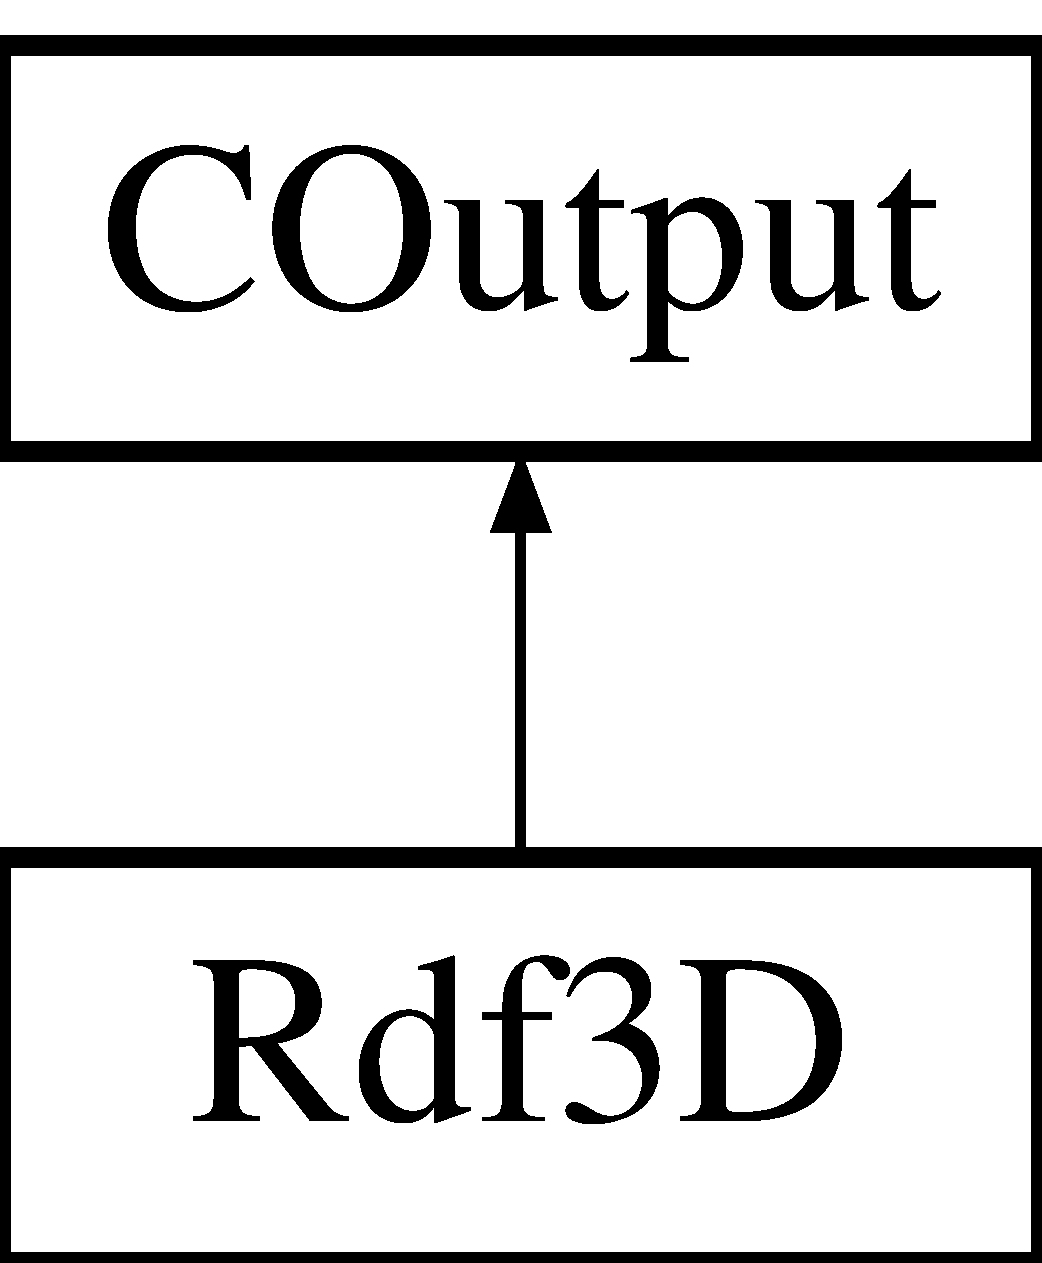
\includegraphics[height=2.000000cm]{classRdf3D}
\end{center}
\end{figure}
\subsection*{Public Member Functions}
\begin{DoxyCompactItemize}
\item 
void \mbox{\hyperlink{classRdf3D_aa86b927b22b369cd1d6ead93c17e43ee}{init\+R\+D\+F3D}} (class \mbox{\hyperlink{classCMolecularSystem}{C\+Molecular\+System}} \&mol\+Sys, double binwidth, double max\+\_\+radius=-\/1.\+0, double volume=-\/1.\+0)
\item 
void \mbox{\hyperlink{classRdf3D_a27efc547d859576b41a16d98cd2d1df9}{single\+R\+D\+F3D}} (class \mbox{\hyperlink{classCMolecularSystem}{C\+Molecular\+System}} \&mol\+Sys, int typeA=-\/1, int typeB=-\/1)
\item 
void \mbox{\hyperlink{classRdf3D_aca3e0b2da042856d705b4bca8f6be335}{accumulate\+R\+D\+F3D}} (class \mbox{\hyperlink{classCMolecularSystem}{C\+Molecular\+System}} \&mol\+Sys, int typeA=-\/1, int typeB=-\/1)
\item 
void \mbox{\hyperlink{classRdf3D_a08d573ef51fd88bd42456a76fc3d7ca4}{normalize\+R\+D\+F3D}} ()
\item 
void \mbox{\hyperlink{classRdf3D_ade47a2d360bcc0112f0da45baef6e609}{getR}} ()
\item 
void \mbox{\hyperlink{classRdf3D_afff83789d5d90cd9cdbf9f7287cd785a}{clear\+R\+D\+F3D}} ()
\item 
void \mbox{\hyperlink{classRdf3D_a76fdc87564a586883c4f290fff3172b2}{print\+R\+D\+F3D}} ()
\item 
void \mbox{\hyperlink{classRdf3D_a6af1bf5b0301a6b43d9f0fffdb868c9c}{delete\+R\+D\+F3D}} ()
\end{DoxyCompactItemize}
\subsection*{Public Attributes}
\begin{DoxyCompactItemize}
\item 
\mbox{\Hypertarget{classRdf3D_a397a94eadf1358d9a1ee57dd02cd58d9}\label{classRdf3D_a397a94eadf1358d9a1ee57dd02cd58d9}} 
double $\ast$ {\bfseries rdf3D}
\item 
\mbox{\Hypertarget{classRdf3D_a2b63db62e5c1839bf611494cd0c0d666}\label{classRdf3D_a2b63db62e5c1839bf611494cd0c0d666}} 
double $\ast$ {\bfseries r\+Val}
\item 
\mbox{\Hypertarget{classRdf3D_a1ac5b0e7ccd247d94ba8188b5dfdd903}\label{classRdf3D_a1ac5b0e7ccd247d94ba8188b5dfdd903}} 
int {\bfseries typeA}
\item 
\mbox{\Hypertarget{classRdf3D_a843c579785b263e64513e88cd9e3b18c}\label{classRdf3D_a843c579785b263e64513e88cd9e3b18c}} 
int {\bfseries typeB}
\end{DoxyCompactItemize}


\subsection{Detailed Description}
Class for 3D R\+DF. This class creates an object for the 3D-\/\+R\+DF, and the output of the R\+DF can be printed to a file. 

Use \mbox{\hyperlink{classRdf3D_aa86b927b22b369cd1d6ead93c17e43ee}{init\+R\+D\+F3\+D()}} to create an object for the 3D R\+DF. Depending on the number of frames, use \mbox{\hyperlink{classRdf3D_a27efc547d859576b41a16d98cd2d1df9}{single\+R\+D\+F3\+D()}} or \mbox{\hyperlink{classRdf3D_aca3e0b2da042856d705b4bca8f6be335}{accumulate\+R\+D\+F3\+D()}} . In case you have used the accumulate function, you will have to use the \mbox{\hyperlink{classRdf3D_a08d573ef51fd88bd42456a76fc3d7ca4}{normalize\+R\+D\+F3\+D()}} to normalize the R\+DF. Finally, print the output to an output file, which is called rdf3\+D.\+txt by default using the print function 

\subsection{Member Function Documentation}
\mbox{\Hypertarget{classRdf3D_aca3e0b2da042856d705b4bca8f6be335}\label{classRdf3D_aca3e0b2da042856d705b4bca8f6be335}} 
\index{Rdf3D@{Rdf3D}!accumulate\+R\+D\+F3D@{accumulate\+R\+D\+F3D}}
\index{accumulate\+R\+D\+F3D@{accumulate\+R\+D\+F3D}!Rdf3D@{Rdf3D}}
\subsubsection{\texorpdfstring{accumulate\+R\+D\+F3\+D()}{accumulateRDF3D()}}
{\footnotesize\ttfamily void Rdf3\+D\+::accumulate\+R\+D\+F3D (\begin{DoxyParamCaption}\item[{class \mbox{\hyperlink{classCMolecularSystem}{C\+Molecular\+System}} \&}]{mol\+Sys,  }\item[{int}]{typeA = {\ttfamily -\/1},  }\item[{int}]{typeB = {\ttfamily -\/1} }\end{DoxyParamCaption})}

Calculates the 3D radial distribution function for a number of snapshots

It accepts the \mbox{\hyperlink{classCMolecularSystem}{C\+Molecular\+System}} object reference and a pair of int type numbers corresponding to lammps type I\+Ds in the trajectory file as arguments. If the integer type I\+Ds are not set, then the R\+DF is calculated for all the atoms in the frame, assuming they are all of the same type.

There is no need to use \mbox{\hyperlink{classRdf3D_a27efc547d859576b41a16d98cd2d1df9}{single\+R\+D\+F3\+D()}} if the R\+DF is to be calculated over a number of frames. You will have to call the normalize function \mbox{\hyperlink{classRdf3D_a08d573ef51fd88bd42456a76fc3d7ca4}{normalize\+R\+D\+F3\+D()}} separately after accumulating to get the R\+DF \mbox{\Hypertarget{classRdf3D_afff83789d5d90cd9cdbf9f7287cd785a}\label{classRdf3D_afff83789d5d90cd9cdbf9f7287cd785a}} 
\index{Rdf3D@{Rdf3D}!clear\+R\+D\+F3D@{clear\+R\+D\+F3D}}
\index{clear\+R\+D\+F3D@{clear\+R\+D\+F3D}!Rdf3D@{Rdf3D}}
\subsubsection{\texorpdfstring{clear\+R\+D\+F3\+D()}{clearRDF3D()}}
{\footnotesize\ttfamily void Rdf3\+D\+::clear\+R\+D\+F3D (\begin{DoxyParamCaption}{ }\end{DoxyParamCaption})}

Sets all the histogram values to zero and sets the number of frames to zero so that the object can be re-\/used. However, the binwidth and maximum radius remain the same. This can be used to re-\/use the object for a different frame etc. Use \mbox{\hyperlink{classRdf3D_a27efc547d859576b41a16d98cd2d1df9}{single\+R\+D\+F3\+D()}} or \mbox{\hyperlink{classRdf3D_aca3e0b2da042856d705b4bca8f6be335}{accumulate\+R\+D\+F3\+D()}} after this function \mbox{\Hypertarget{classRdf3D_a6af1bf5b0301a6b43d9f0fffdb868c9c}\label{classRdf3D_a6af1bf5b0301a6b43d9f0fffdb868c9c}} 
\index{Rdf3D@{Rdf3D}!delete\+R\+D\+F3D@{delete\+R\+D\+F3D}}
\index{delete\+R\+D\+F3D@{delete\+R\+D\+F3D}!Rdf3D@{Rdf3D}}
\subsubsection{\texorpdfstring{delete\+R\+D\+F3\+D()}{deleteRDF3D()}}
{\footnotesize\ttfamily void Rdf3\+D\+::delete\+R\+D\+F3D (\begin{DoxyParamCaption}{ }\end{DoxyParamCaption})}

Frees the memory \mbox{\Hypertarget{classRdf3D_ade47a2d360bcc0112f0da45baef6e609}\label{classRdf3D_ade47a2d360bcc0112f0da45baef6e609}} 
\index{Rdf3D@{Rdf3D}!getR@{getR}}
\index{getR@{getR}!Rdf3D@{Rdf3D}}
\subsubsection{\texorpdfstring{get\+R()}{getR()}}
{\footnotesize\ttfamily void Rdf3\+D\+::getR (\begin{DoxyParamCaption}{ }\end{DoxyParamCaption})}

Get the radial R values corresponding to each R\+DF value This will remain the same over all frames \mbox{\Hypertarget{classRdf3D_aa86b927b22b369cd1d6ead93c17e43ee}\label{classRdf3D_aa86b927b22b369cd1d6ead93c17e43ee}} 
\index{Rdf3D@{Rdf3D}!init\+R\+D\+F3D@{init\+R\+D\+F3D}}
\index{init\+R\+D\+F3D@{init\+R\+D\+F3D}!Rdf3D@{Rdf3D}}
\subsubsection{\texorpdfstring{init\+R\+D\+F3\+D()}{initRDF3D()}}
{\footnotesize\ttfamily void Rdf3\+D\+::init\+R\+D\+F3D (\begin{DoxyParamCaption}\item[{class \mbox{\hyperlink{classCMolecularSystem}{C\+Molecular\+System}} \&}]{mol\+Sys,  }\item[{double}]{binwidth,  }\item[{double}]{max\+\_\+radius = {\ttfamily -\/1.0},  }\item[{double}]{volume = {\ttfamily -\/1.0} }\end{DoxyParamCaption})}

Initializes the histogram array for 3-\/D R\+DF

It takes the \mbox{\hyperlink{classCMolecularSystem}{C\+Molecular\+System}} object reference and binwidth as arguments. Optional arguments include the maximum radius upto which the 3-\/D R\+DF will be calculated and the desired volume. If not set, the default values are half the simulation box and the volume of the simulation box respectively \mbox{\Hypertarget{classRdf3D_a08d573ef51fd88bd42456a76fc3d7ca4}\label{classRdf3D_a08d573ef51fd88bd42456a76fc3d7ca4}} 
\index{Rdf3D@{Rdf3D}!normalize\+R\+D\+F3D@{normalize\+R\+D\+F3D}}
\index{normalize\+R\+D\+F3D@{normalize\+R\+D\+F3D}!Rdf3D@{Rdf3D}}
\subsubsection{\texorpdfstring{normalize\+R\+D\+F3\+D()}{normalizeRDF3D()}}
{\footnotesize\ttfamily void Rdf3\+D\+::normalize\+R\+D\+F3D (\begin{DoxyParamCaption}{ }\end{DoxyParamCaption})}

Normalizes the R\+DF

You will have to call this after \mbox{\hyperlink{classRdf3D_aca3e0b2da042856d705b4bca8f6be335}{accumulate\+R\+D\+F3\+D()}} if you are averaging over several snapshots. This is automatically called inside single\+R\+D\+F3D \mbox{\Hypertarget{classRdf3D_a76fdc87564a586883c4f290fff3172b2}\label{classRdf3D_a76fdc87564a586883c4f290fff3172b2}} 
\index{Rdf3D@{Rdf3D}!print\+R\+D\+F3D@{print\+R\+D\+F3D}}
\index{print\+R\+D\+F3D@{print\+R\+D\+F3D}!Rdf3D@{Rdf3D}}
\subsubsection{\texorpdfstring{print\+R\+D\+F3\+D()}{printRDF3D()}}
{\footnotesize\ttfamily void Rdf3\+D\+::print\+R\+D\+F3D (\begin{DoxyParamCaption}{ }\end{DoxyParamCaption})}

Prints out the 3D R\+DF function to a file in the output folder \mbox{\Hypertarget{classRdf3D_a27efc547d859576b41a16d98cd2d1df9}\label{classRdf3D_a27efc547d859576b41a16d98cd2d1df9}} 
\index{Rdf3D@{Rdf3D}!single\+R\+D\+F3D@{single\+R\+D\+F3D}}
\index{single\+R\+D\+F3D@{single\+R\+D\+F3D}!Rdf3D@{Rdf3D}}
\subsubsection{\texorpdfstring{single\+R\+D\+F3\+D()}{singleRDF3D()}}
{\footnotesize\ttfamily void Rdf3\+D\+::single\+R\+D\+F3D (\begin{DoxyParamCaption}\item[{class \mbox{\hyperlink{classCMolecularSystem}{C\+Molecular\+System}} \&}]{mol\+Sys,  }\item[{int}]{typeA = {\ttfamily -\/1},  }\item[{int}]{typeB = {\ttfamily -\/1} }\end{DoxyParamCaption})}

Calculates the 3D radial distribution function for a single snapshot Use this only if there is one frame only.

It accepts a pair of int type numbers corresponding to lammps type I\+Ds in the trajectory file as arguments. If the integer type I\+Ds are not set, then the R\+DF is calculated for all the atoms in the frame, assuming they are all of the same type. 

The documentation for this class was generated from the following files\+:\begin{DoxyCompactItemize}
\item 
rdf3\+D.\+h\item 
rdf3\+D.\+cpp\end{DoxyCompactItemize}

\hypertarget{structs__rawParameter}{}\section{s\+\_\+raw\+Parameter Struct Reference}
\label{structs__rawParameter}\index{s\+\_\+raw\+Parameter@{s\+\_\+raw\+Parameter}}
\subsection*{Public Attributes}
\begin{DoxyCompactItemize}
\item 
\mbox{\Hypertarget{structs__rawParameter_adc33c81f18be5e4a799018b4bbaabe82}\label{structs__rawParameter_adc33c81f18be5e4a799018b4bbaabe82}} 
std\+::string {\bfseries name}
\item 
\mbox{\Hypertarget{structs__rawParameter_a8309e9f3e4b26f6629638a80a82788ba}\label{structs__rawParameter_a8309e9f3e4b26f6629638a80a82788ba}} 
std\+::string {\bfseries value}
\end{DoxyCompactItemize}


The documentation for this struct was generated from the following file\+:\begin{DoxyCompactItemize}
\item 
parameter.\+h\end{DoxyCompactItemize}

%--- End generated contents ---

% Index
\backmatter
\newpage
\phantomsection
\clearemptydoublepage
\addcontentsline{toc}{chapter}{Index}
\printindex

\end{document}
